% Options for packages loaded elsewhere
\PassOptionsToPackage{unicode}{hyperref}
\PassOptionsToPackage{hyphens}{url}
\PassOptionsToPackage{dvipsnames,svgnames,x11names}{xcolor}
%
\documentclass[
  letterpaper,
  DIV=11,
  numbers=noendperiod]{scrartcl}

\usepackage{amsmath,amssymb}
\usepackage{lmodern}
\usepackage{iftex}
\ifPDFTeX
  \usepackage[T1]{fontenc}
  \usepackage[utf8]{inputenc}
  \usepackage{textcomp} % provide euro and other symbols
\else % if luatex or xetex
  \usepackage{unicode-math}
  \defaultfontfeatures{Scale=MatchLowercase}
  \defaultfontfeatures[\rmfamily]{Ligatures=TeX,Scale=1}
\fi
% Use upquote if available, for straight quotes in verbatim environments
\IfFileExists{upquote.sty}{\usepackage{upquote}}{}
\IfFileExists{microtype.sty}{% use microtype if available
  \usepackage[]{microtype}
  \UseMicrotypeSet[protrusion]{basicmath} % disable protrusion for tt fonts
}{}
\makeatletter
\@ifundefined{KOMAClassName}{% if non-KOMA class
  \IfFileExists{parskip.sty}{%
    \usepackage{parskip}
  }{% else
    \setlength{\parindent}{0pt}
    \setlength{\parskip}{6pt plus 2pt minus 1pt}}
}{% if KOMA class
  \KOMAoptions{parskip=half}}
\makeatother
\usepackage{xcolor}
\setlength{\emergencystretch}{3em} % prevent overfull lines
\setcounter{secnumdepth}{-\maxdimen} % remove section numbering
% Make \paragraph and \subparagraph free-standing
\ifx\paragraph\undefined\else
  \let\oldparagraph\paragraph
  \renewcommand{\paragraph}[1]{\oldparagraph{#1}\mbox{}}
\fi
\ifx\subparagraph\undefined\else
  \let\oldsubparagraph\subparagraph
  \renewcommand{\subparagraph}[1]{\oldsubparagraph{#1}\mbox{}}
\fi


\providecommand{\tightlist}{%
  \setlength{\itemsep}{0pt}\setlength{\parskip}{0pt}}\usepackage{longtable,booktabs,array}
\usepackage{calc} % for calculating minipage widths
% Correct order of tables after \paragraph or \subparagraph
\usepackage{etoolbox}
\makeatletter
\patchcmd\longtable{\par}{\if@noskipsec\mbox{}\fi\par}{}{}
\makeatother
% Allow footnotes in longtable head/foot
\IfFileExists{footnotehyper.sty}{\usepackage{footnotehyper}}{\usepackage{footnote}}
\makesavenoteenv{longtable}
\usepackage{graphicx}
\makeatletter
\def\maxwidth{\ifdim\Gin@nat@width>\linewidth\linewidth\else\Gin@nat@width\fi}
\def\maxheight{\ifdim\Gin@nat@height>\textheight\textheight\else\Gin@nat@height\fi}
\makeatother
% Scale images if necessary, so that they will not overflow the page
% margins by default, and it is still possible to overwrite the defaults
% using explicit options in \includegraphics[width, height, ...]{}
\setkeys{Gin}{width=\maxwidth,height=\maxheight,keepaspectratio}
% Set default figure placement to htbp
\makeatletter
\def\fps@figure{htbp}
\makeatother
\newlength{\cslhangindent}
\setlength{\cslhangindent}{1.5em}
\newlength{\csllabelwidth}
\setlength{\csllabelwidth}{3em}
\newlength{\cslentryspacingunit} % times entry-spacing
\setlength{\cslentryspacingunit}{\parskip}
\newenvironment{CSLReferences}[2] % #1 hanging-ident, #2 entry spacing
 {% don't indent paragraphs
  \setlength{\parindent}{0pt}
  % turn on hanging indent if param 1 is 1
  \ifodd #1
  \let\oldpar\par
  \def\par{\hangindent=\cslhangindent\oldpar}
  \fi
  % set entry spacing
  \setlength{\parskip}{#2\cslentryspacingunit}
 }%
 {}
\usepackage{calc}
\newcommand{\CSLBlock}[1]{#1\hfill\break}
\newcommand{\CSLLeftMargin}[1]{\parbox[t]{\csllabelwidth}{#1}}
\newcommand{\CSLRightInline}[1]{\parbox[t]{\linewidth - \csllabelwidth}{#1}\break}
\newcommand{\CSLIndent}[1]{\hspace{\cslhangindent}#1}

\KOMAoption{captions}{tableheading}
\makeatletter
\makeatother
\makeatletter
\makeatother
\makeatletter
\@ifpackageloaded{caption}{}{\usepackage{caption}}
\AtBeginDocument{%
\ifdefined\contentsname
  \renewcommand*\contentsname{Table of contents}
\else
  \newcommand\contentsname{Table of contents}
\fi
\ifdefined\listfigurename
  \renewcommand*\listfigurename{List of Figures}
\else
  \newcommand\listfigurename{List of Figures}
\fi
\ifdefined\listtablename
  \renewcommand*\listtablename{List of Tables}
\else
  \newcommand\listtablename{List of Tables}
\fi
\ifdefined\figurename
  \renewcommand*\figurename{Figure}
\else
  \newcommand\figurename{Figure}
\fi
\ifdefined\tablename
  \renewcommand*\tablename{Table}
\else
  \newcommand\tablename{Table}
\fi
}
\@ifpackageloaded{float}{}{\usepackage{float}}
\floatstyle{ruled}
\@ifundefined{c@chapter}{\newfloat{codelisting}{h}{lop}}{\newfloat{codelisting}{h}{lop}[chapter]}
\floatname{codelisting}{Listing}
\newcommand*\listoflistings{\listof{codelisting}{List of Listings}}
\makeatother
\makeatletter
\@ifpackageloaded{caption}{}{\usepackage{caption}}
\@ifpackageloaded{subcaption}{}{\usepackage{subcaption}}
\makeatother
\makeatletter
\@ifpackageloaded{tcolorbox}{}{\usepackage[many]{tcolorbox}}
\makeatother
\makeatletter
\@ifundefined{shadecolor}{\definecolor{shadecolor}{rgb}{.97, .97, .97}}
\makeatother
\makeatletter
\makeatother
\ifLuaTeX
  \usepackage{selnolig}  % disable illegal ligatures
\fi
\IfFileExists{bookmark.sty}{\usepackage{bookmark}}{\usepackage{hyperref}}
\IfFileExists{xurl.sty}{\usepackage{xurl}}{} % add URL line breaks if available
\urlstyle{same} % disable monospaced font for URLs
\hypersetup{
  pdfauthor={Amanda Dumi},
  colorlinks=true,
  linkcolor={blue},
  filecolor={Maroon},
  citecolor={Blue},
  urlcolor={Blue},
  pdfcreator={LaTeX via pandoc}}

\author{Amanda Dumi}
\date{}

\begin{document}
\ifdefined\Shaded\renewenvironment{Shaded}{\begin{tcolorbox}[interior hidden, frame hidden, breakable, enhanced, boxrule=0pt, sharp corners, borderline west={3pt}{0pt}{shadecolor}]}{\end{tcolorbox}}\fi

\newcommand{\bra}[1]{\left<#1\right|}\newcommand{\ket}[1]{\left|#1\right>}\newcommand{\bk}[2]{\left<#1\middle|#2\right>}\newcommand{\bke}[3]{\left<#1\middle|#2\middle|#3\right>}

Reliable approximation in electronic structure methods:

from real space partitioning to quantum Monte Carlo approaches

Amanda Dumi Seminar at Oak Ridge National Laboratory

\hypertarget{current_date}{}

\begin{center}\rule{0.5\linewidth}{0.5pt}\end{center}

When is DFT not enough?

\begin{itemize}
\tightlist
\item
  DFT citation/publications demonstrate it's applicability and often
  reliable performance
\item
  In strongly correlated regimes, or when functional and system physics
  do not agree
\end{itemize}

\begin{center}\rule{0.5\linewidth}{0.5pt}\end{center}

Reduce cost through various system reductions

\textbf{Sampling Configurations} Quantum Monte Carlo: applications and
developments

\textbf{Hilbert Space}

selected CI as approximate trial wave functions

\textbf{Real Space}

Determining molecular fragments with unsupervised machine learning (UML)

\begin{center}\rule{0.5\linewidth}{0.5pt}\end{center}

QMC application:{ periodic absorption\footnote{A. Dumi et al, {`The
  Binding of Atomic Hydrogen on Graphene from Density Functional Theory
  and Diffusion Monte Carlo Calculations'}, \emph{The Journal of
  Chemical Physics}, 156.14 (2022),
  144702DOI:\href{https://doi.org/10.1063/5.0085982}{10.1063/5.0085982}.}}

H on graphene

\begin{longtable}[]{@{}ll@{}}
\toprule()
Method & Binding energy (meV) \\
\midrule()
\endhead
DMC & -691 \(\pm\) 19 \\
PW91 & -810 to -830, -870 \\
PBE & -790, -840, -980 \\
\bottomrule()
\end{longtable}

\begin{itemize}
\tightlist
\item
  functional dependent binding energy
\item
  a need for benchmark values
\end{itemize}

\begin{center}\rule{0.5\linewidth}{0.5pt}\end{center}

Diffusion Monte Carlo

\begin{itemize}
\item
  Recast the Schrodinger equation in imaginary time

  \[\frac{\partial \left|\Psi\right>}{\partial \tau} = - \hat{H} \left|\Psi\right> \]

  \begin{itemize}
  \tightlist
  \item
    A formal soltuion to this:
  \end{itemize}
\end{itemize}

\[\left|\psi\left(\tau_{1}+\delta \tau\right)\right\rangle=e^{-\hat{H} \delta \tau}\left|\psi\left(\tau_{1}\right)\right\rangle\]

Anything non-orthogonal to the ground state is going to decay out
exponentially

\[\lim _{\tau \rightarrow \infty}|\psi(\tau)\rangle=c_{0} e^{-\epsilon_{0} \tau}\left|\phi_{0}\right\rangle\]

\begin{center}\rule{0.5\linewidth}{0.5pt}\end{center}

\begin{center}\rule{0.5\linewidth}{0.5pt}\end{center}

\[ -\frac{\partial \psi(\mathbf{R}, \tau)}{\partial \tau} = \]

\[\left[\sum_{i=1}^{N}-\frac{1}{2} \nabla_{i}^{2} \psi(\mathbf{R}, \tau)\right] \text{ diffusion term}\]

\[+\]

\[\left(V(\mathbf{R})-E_{T}\right) \psi(\mathbf{R}, \tau) \text{ branching term}\]

\hypertarget{section}{%
\subsection{}\label{section}}

Importance sampling

\begin{itemize}
\tightlist
\item
  use of trial wavefunction for efficient sampling.
\end{itemize}

Fixed-node approximation

\begin{itemize}
\tightlist
\item
  Antisymmetry of fermions causes sampling problems
\item
  Solution: fix nodes of trial wavefunction
\item
  necessitates accurate nodal surface of trial wavefunction
\end{itemize}

\begin{center}\rule{0.5\linewidth}{0.5pt}\end{center}

QMC application:{ periodic absorption}

H on graphene

\begin{longtable}[]{@{}ll@{}}
\toprule()
Method & Binding energy (meV) \\
\midrule()
\endhead
PBE & -820 \\
PBE & -871 \\
PBE0 & -851 (-800) \\
HSE & -794 (-743) \\
DMC & -691 \(\pm\) 19 \\
PW91 & -810 to -830, -870 \\
PBE & -790, -840, -980 \\
\bottomrule()
\end{longtable}

\begin{itemize}
\tightlist
\item
  QMCPACK binding energies provide benchmark.
\item
  Hybrid functionals are very close.
\item
  Even with close binding energies, density seems to disagree in bonding
  region.
\end{itemize}

\begin{center}\rule{0.5\linewidth}{0.5pt}\end{center}

Reduce cost through various system reductions

\textbf{Sampling Configurations} Quantum Monte Carlo: applications and
developments

\textbf{Hilbert Space}

selected CI as approximate trial wave functions

\textbf{Real Space}

Determining molecular fragments with unsupervised machine learning (UML)

\begin{center}\rule{0.5\linewidth}{0.5pt}\end{center}

\leavevmode\vadjust pre{\hypertarget{hilbert_space}{}}%
QMC application:{ non-valence correlation bound anion\footnote{S.
  Upadhyay et al, {`The Role of High-Order Electron Correlation Effects
  in a Model System for Non-Valence Correlation-Bound Anions'},
  \emph{The Journal of Chemical Physics}, 153.22 (2020),
  224118DOI:\href{https://doi.org/10.1063/5.0030942}{10.1063/5.0030942}.}}

NVCB rely on accurate description of correlation to bind

\[E_{corr} = E_{true}-E_{HF}\]

model system: H\(_2\)O\(_4\)

Radial integration of Hartree-Fock orbital density, \(R=4\) Angstroms

\begin{center}\rule{0.5\linewidth}{0.5pt}\end{center}

Selected-CI

\(\Psi_n = \sum c_I^{(n)}\left|D_I\right>\)

\(e_\alpha = \frac{ \langle \Psi^{(n)}| {\hat H} | \alpha \rangle^2 }{E^{(n)} - \langle \alpha | {\hat H} | \alpha \rangle }.\)

\(\{ \left|\alpha\right> \}\)

single \& double excitations

\(\{ \left|\alpha\right> \}_*^{(n)}\)

\(\Psi_n\)

\(\Psi_{n+1}\)

\begin{center}\rule{0.5\linewidth}{0.5pt}\end{center}

H\(_2\)O\(_4\) Results

\begin{longtable}[]{@{}lll@{}}
\toprule()
wave function & basis set & EBE (meV) \\
\midrule()
\endhead
D/HF & aug-cc-pVDZ+7s7p & 183 \(\pm\) 10 \\
SD/HF & aug-cc-pVDZ & 176 \(\pm\) 12 \\
SD/HF & cc-pVDZ & -528 \(\pm\) 25 \\
SD/B3LYP & aug-cc-pVDZ+7s7p & 212 \(\pm\) 11 \\
SD/HF(N)//SD/NO SDCI(A) & aug-cc-pVDZ+7s7p & 205 \(\pm\) 10 \\
SD/HF(N)//MD/NO SDCI(A) & aug-cc-pVDZ+7s7p & 202 \(\pm\) 12 \\
MD/CIPSI NO & aug-cc-pVDZ+3s1p & 190 \(\pm\) 9 \\
\bottomrule()
\end{longtable}

\begin{itemize}
\tightlist
\item
  Summary of selected-CI success/challenges and overall performance of
  other methods.
\end{itemize}

\(R\) = 7

\begin{itemize}
\tightlist
\item
  HF binds electron -\textgreater{} correlation not essential
\item
  still orbital shape has noticeable changes
\item
  DFT can recover those changes.
\end{itemize}

\(R\) = 4

\begin{itemize}
\tightlist
\item
  NCVB regime
\item
  HF does not bind
\item
  CIPSI shape changes slight, impacts energy.
\item
  SDCI shape seems wrong
\end{itemize}

\begin{center}\rule{0.5\linewidth}{0.5pt}\end{center}

\leavevmode\vadjust pre{\hypertarget{hilbert_space}{}}%
Follow-up Questions {Ongoing projects at Sandia National Laboratories }

\begin{itemize}
\tightlist
\item
  Can various selected CI approaches or later optimizations improve the
  compactness and quality of the trial wave function?
\end{itemize}

\begin{itemize}
\tightlist
\item
  Is there a balance in how well we are capturing dynamic vs static
  correlation in these systems? Especially in cases of energy
  differences.
\end{itemize}

\(\hookrightarrow\) Aluminum systematic study: exploring various
multideterminant generation and optimization schemes

\begin{itemize}
\tightlist
\item
  Selected CI captures static correlation, but should we take a second
  look at how dynamic correlation is captured?
\end{itemize}

{ \(\hookrightarrow\) Jastrow form study}

\begin{center}\rule{0.5\linewidth}{0.5pt}\end{center}

Jastrow Factor forms

\[\Psi(\{r_i\}\{r_I\})=exp(\mathcal{J})D(\{r_{i}\})\]

standard: parameterize separate 1,2, and 2-body terms. optimize
parameters with VMC

\textbf{A possible alternative form:}

\begin{itemize}
\item
  Using framework of SNAP atomic potential
\item
  represent the particle densities as bispectrum components.\footnote{A.
    P. Bartók, R. Kondor, and G. Csányi, {`On Representing Chemical
    Environments'}, \emph{Phys. Rev. B}, 87 (2013),
    184115DOI:\href{https://doi.org/10.1103/PhysRevB.87.184115}{10.1103/PhysRevB.87.184115}.}
  \footnote{,A. P. Thompson et al, {`Spectral Neighbor Analysis Method
    for Automated Generation of Quantum-Accurate Interatomic
    Potentials'}, \emph{Journal of Computational Physics}, 285 (2015),
    316--30DOI:\url{https://doi.org/10.1016/j.jcp.2014.12.018}.}
\item
  A perspective of particle neighborhoods which require fewer parameters
  for VMC optimization
\end{itemize}

\begin{center}\rule{0.5\linewidth}{0.5pt}\end{center}

Projection of the \(\rho\) particle density on the surface of the 4-D
sphere:

\[E_{S N A P}^{i}\left(\mathbf{B}^{i}\right)=\beta_{0}^{\alpha_{i}}+\sum_{k=1}^K \beta_{k}^{\alpha_{i}} B_{k}^{i}=\beta_{0}^{\alpha_{i}}+\beta^{\alpha_{i}} \cdot \mathbf{B}^{i}\]

\[\begin{aligned} B_{j_{1}, j_{2}, j}=& \sum_{m_{1}^{\prime}, m_{1}=-j_{1}}^{j_{1}} \sum_{m_{2}^{\prime}, m_{2}=-j_{2}}^{j_{2}} \sum_{m^{\prime}, m=-j}^{j}\left(c_{m^{\prime} m}^{j}\right)^{*} C_{j_{1} m_{1} j_{2} m_{2}}^{j m} \\ & \times C_{j_{1} m_{1}^{\prime} j_{2} m_{2}^{\prime}}^{j m^{\prime}} c_{m_{1}^{\prime} m_{1}}^{j_{1}} c_{m_{2}^{\prime} m_{2}}^{j_{2}} \end{aligned}\]

TO DO:

initial python sandbox for testing unit tests ensure single and multiple
species work accessing LAMMPS API object interface with QMCPack

\begin{center}\rule{0.5\linewidth}{0.5pt}\end{center}

Reduce cost through various system reductions

\textbf{Sampling Configurations} Quantum Monte Carlo: applications and
developments

\textbf{Hilbert Space}

selected CI as approximate trial wave functions

\textbf{Real Space}

Determining molecular fragments with unsupervised machine learning (UML)

\begin{center}\rule{0.5\linewidth}{0.5pt}\end{center}

\leavevmode\vadjust pre{\hypertarget{real_space}{}}%
Fragmenting with unsupervised machine learning

Problem

\begin{figure}

{\centering \includegraphics[width=0.6\textwidth,height=\textheight]{images/large_polymer_example.png}

}

\end{figure}

\begin{center}\rule{0.5\linewidth}{0.5pt}\end{center}

\leavevmode\vadjust pre{\hypertarget{real_space}{}}%
Fragmenting with unsupervised machine learning

Problem

\begin{figure}

{\centering \includegraphics[width=0.8\textwidth,height=\textheight]{images/large_polymer_example.png}

}

\end{figure}

Approach

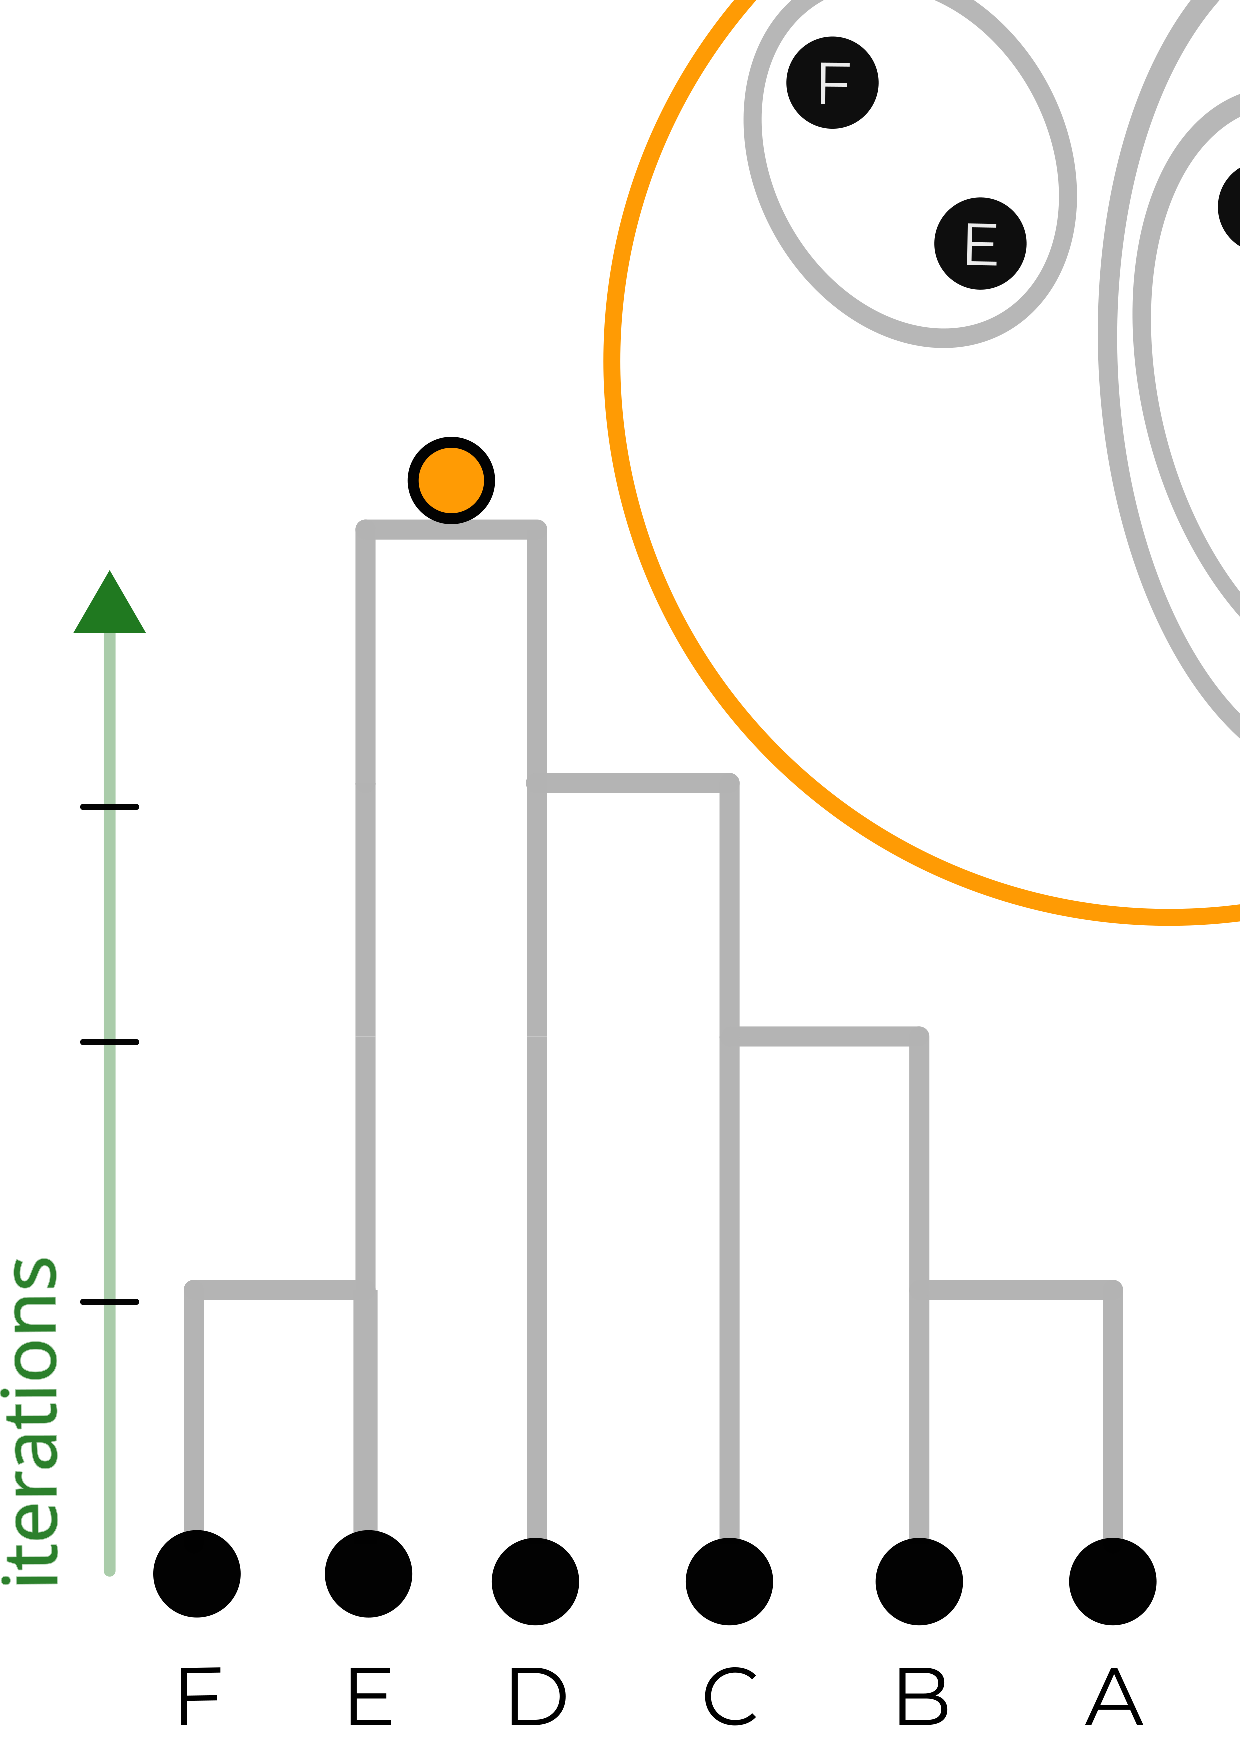
\includegraphics[width=0.95\textwidth,height=\textheight]{images/methods.png}

\includegraphics[width=0.95\textwidth,height=\textheight]{images/descriptors.png}

\begin{center}\rule{0.5\linewidth}{0.5pt}\end{center}

Performance

Systems:

\begin{itemize}
\tightlist
\item
  water clusters
\item
  methylthiophenes
\item
  small polymer systems
\end{itemize}

Performance:

\begin{figure}

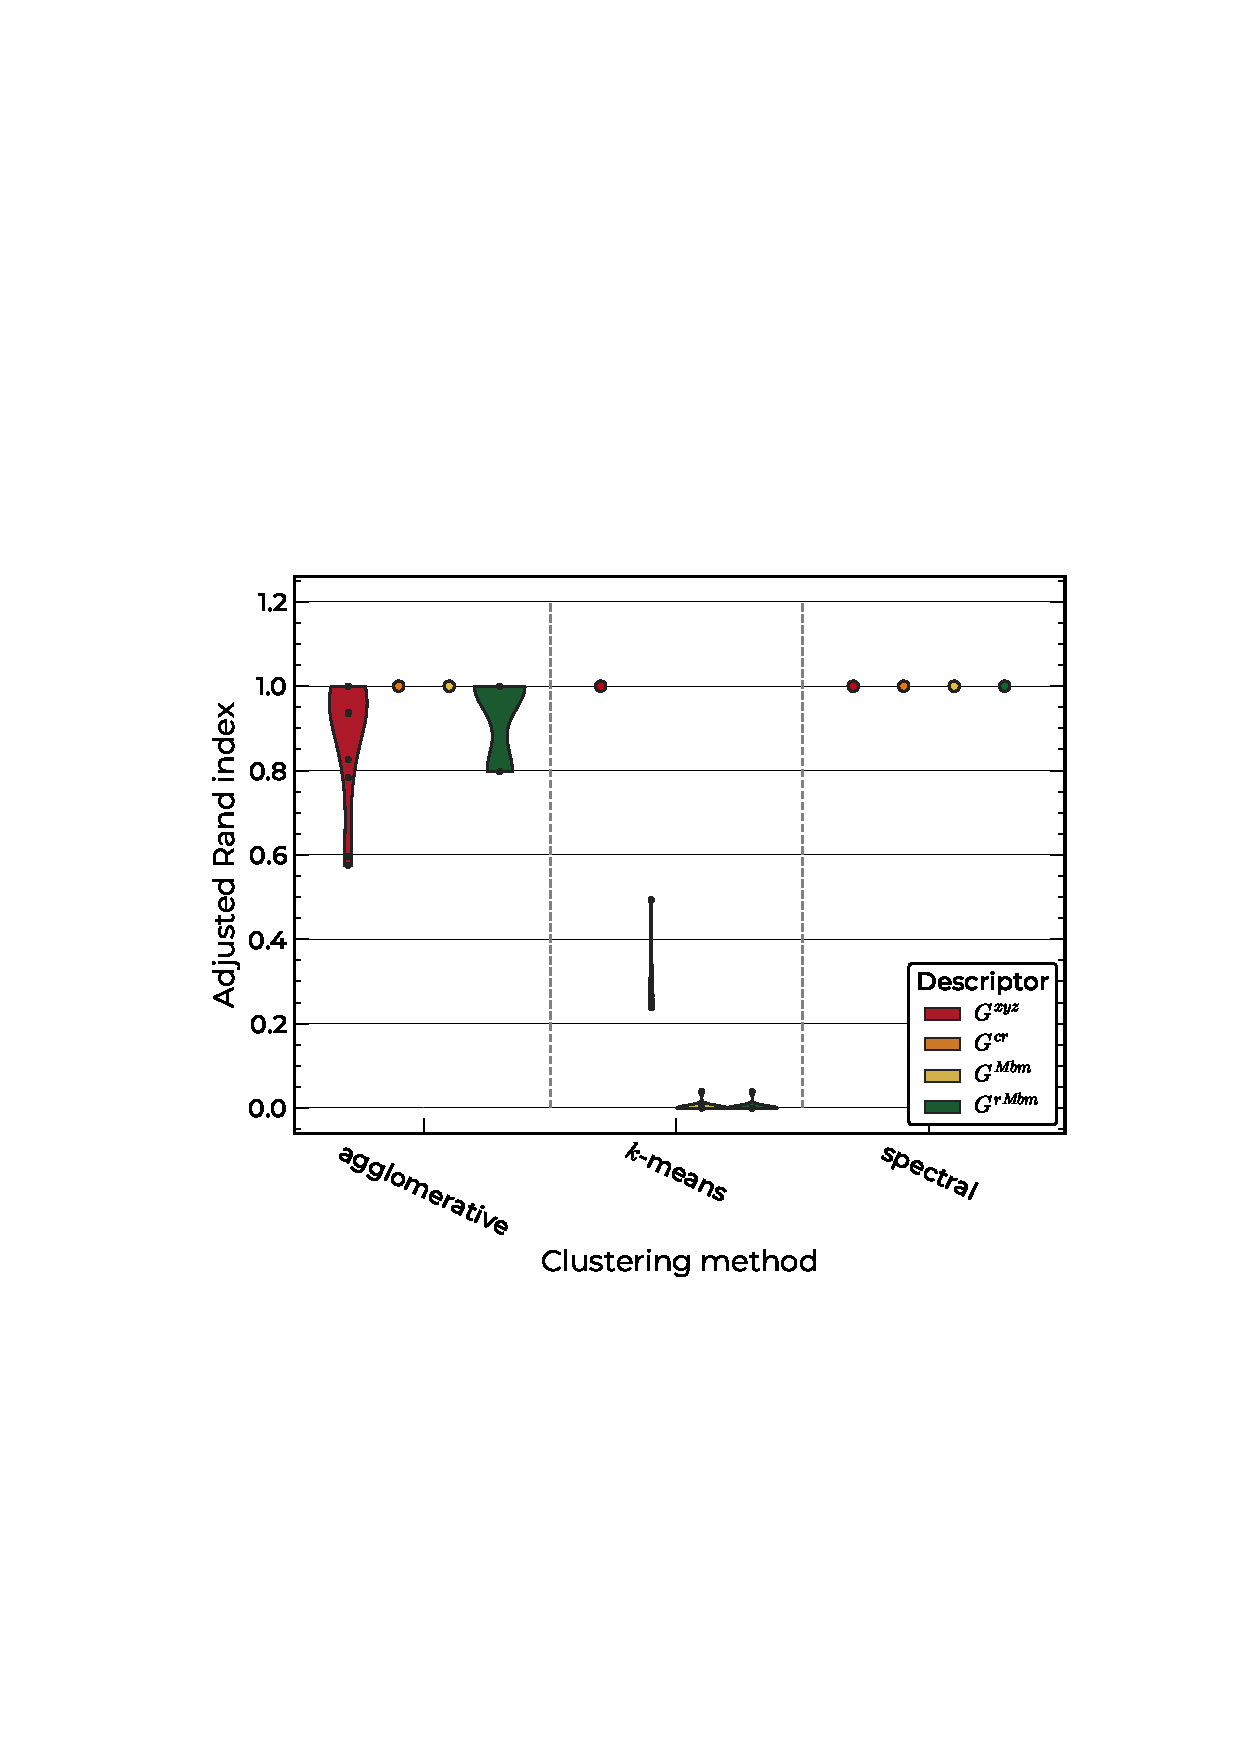
\includegraphics[width=0.5\textwidth,height=\textheight]{images/mt_wb97x-d_violin_randidx.png} \hfill{}

\end{figure}

Summary:

\begin{itemize}
\tightlist
\item
  UML methods are able to resolve fragments
\item
  spectral clustering performs well and is insensitive to descriptor
\end{itemize}

\begin{center}\rule{0.5\linewidth}{0.5pt}\end{center}

Acknowledgements

\begin{itemize}
\tightlist
\item
  Dr.~Kenneth D. Jordan
\item
  Dr.~Daniel S. Lambrecht
\item
  Dr.~Luke Shulenburger, Dr.~Raymond Clay
\end{itemize}

Computational Resources

\begin{itemize}
\tightlist
\item
  Center for Research computing, University of Pittsburgh
\item
  Argonne Leadership Computing Facility
\item
  Sandia National Laboratories
\end{itemize}

Funding:

\begin{itemize}
\tightlist
\item
  ACS: DNI-63213
\item
  NSF: 1807638
\item
  Sandia National Laboratories is a multimission laboratory managed and
  operated by National Technology \& Engineering Solutions of Sandia,
  LLC, a wholly owned subsidiary of Honeywell International Inc., for
  the U.S. Department of Energy's National Nuclear Security
  Administration under contract DE-NA0003525.
\end{itemize}

\begin{center}\rule{0.5\linewidth}{0.5pt}\end{center}

\hypertarget{conclusions}{%
\subsection{Conclusions}\label{conclusions}}

In regimes of strong electron correlation, mean field methods may be
problematic and require need alternatives

Presented on three approaches:

\begin{itemize}
\tightlist
\item
  QMC: application to H\(_2\)O\(_4\) and H on graphene
  \(\hookrightarrow\) systems where DFT varies.
\item
  SCI methods in H\(_2\)O\(_4\) as trial wave function
\item
  UML MF: offer an approach to determining molecular fragmentation
  automatically, with very little information
\end{itemize}

\begin{center}\rule{0.5\linewidth}{0.5pt}\end{center}

References

\hypertarget{refs}{}
\begin{CSLReferences}{1}{0}
\leavevmode\vadjust pre{\hypertarget{ref-PhysRevB.87.184115}{}}%
Albert P. Bartók, Risi Kondor, \& Gábor Csányi, {`On Representing
Chemical Environments'}, \emph{Phys. Rev. B}, 87 (2013),
184115DOI:\href{https://doi.org/10.1103/PhysRevB.87.184115}{10.1103/PhysRevB.87.184115}

\leavevmode\vadjust pre{\hypertarget{ref-doi:10.1063ux2f5.0085982}{}}%
Amanda Dumi, Shiv Upadhyay, Leonardo Bernasconi, Hyeondeok Shin, Anouar
Benali, \& Kenneth D. Jordan, {`The Binding of Atomic Hydrogen on
Graphene from Density Functional Theory and Diffusion Monte Carlo
Calculations'}, \emph{The Journal of Chemical Physics}, 156.14 (2022),
144702DOI:\href{https://doi.org/10.1063/5.0085982}{10.1063/5.0085982}

\leavevmode\vadjust pre{\hypertarget{ref-THOMPSON2015316}{}}%
A. P. Thompson, L. P. Swiler, C. R. Trott, S. M. Foiles, \& G. J.
Tucker, {`Spectral Neighbor Analysis Method for Automated Generation of
Quantum-Accurate Interatomic Potentials'}, \emph{Journal of
Computational Physics}, 285 (2015),
316--30DOI:\url{https://doi.org/10.1016/j.jcp.2014.12.018}

\leavevmode\vadjust pre{\hypertarget{ref-doi:10.1063ux2f5.0030942}{}}%
Shiv Upadhyay, Amanda Dumi, James Shee, \& Kenneth D. Jordan, {`The Role
of High-Order Electron Correlation Effects in a Model System for
Non-Valence Correlation-Bound Anions'}, \emph{The Journal of Chemical
Physics}, 153.22 (2020),
224118DOI:\href{https://doi.org/10.1063/5.0030942}{10.1063/5.0030942}

\end{CSLReferences}



\end{document}
